\documentclass{article}
\usepackage[spanish]{babel}
\usepackage[utf8]{inputenc}
\usepackage[T1]{fontenc}
\usepackage{hyperref}
\usepackage{xcolor}
\usepackage{listings}
\usepackage{minted}
\usepackage{graphicx}
\hypersetup{
    colorlinks,
    linkcolor={red!50!black},
    citecolor={blue!50!black},
    urlcolor={blue!80!black}
}

\title{P1: Desarrollo de una Web}
\author{Daniel Ramos}
\date{\today}

\begin{document}

\maketitle

\begin{center}
    \large Herramientas HTML y CSS I
\end{center}

\newpage

\tableofcontents

\newpage

\section*{Introducción}
En esta práctica, aprenderemos a configurar el entorno de desarrollo necesario para trabajar con HTML y CSS. Esto incluye la instalación de editores de texto, navegadores web y otras herramientas útiles.

\newpage

\section{Configurando el Entorno de Desarrollo}

El primer paso ha sido inicializar el repositorio en el que se hará el desarrollo de la práctica con \lstinline|git init| y \lstinline|npm init|.

Siguiendo la guía de la web de parcel, lo siguiente ha sido instalar Parcel como dependencia del proyecto con \lstinline|npm install --save-dev parcel|.

Una vez instalado Parcel, se ha probado su correcto funcionamiento creando un \textit{Hello World}. Una vez creado el fichero \lstinline|src/index.html| se ha ejecutado el comando \lstinline|npx parcel src/index.html| y se ha comprobado que la página web de abría correctamente en el navegador como se ve en la Figura~\ref{fig:hello-world}.

 \begin{figure}[h!]
     \centering
     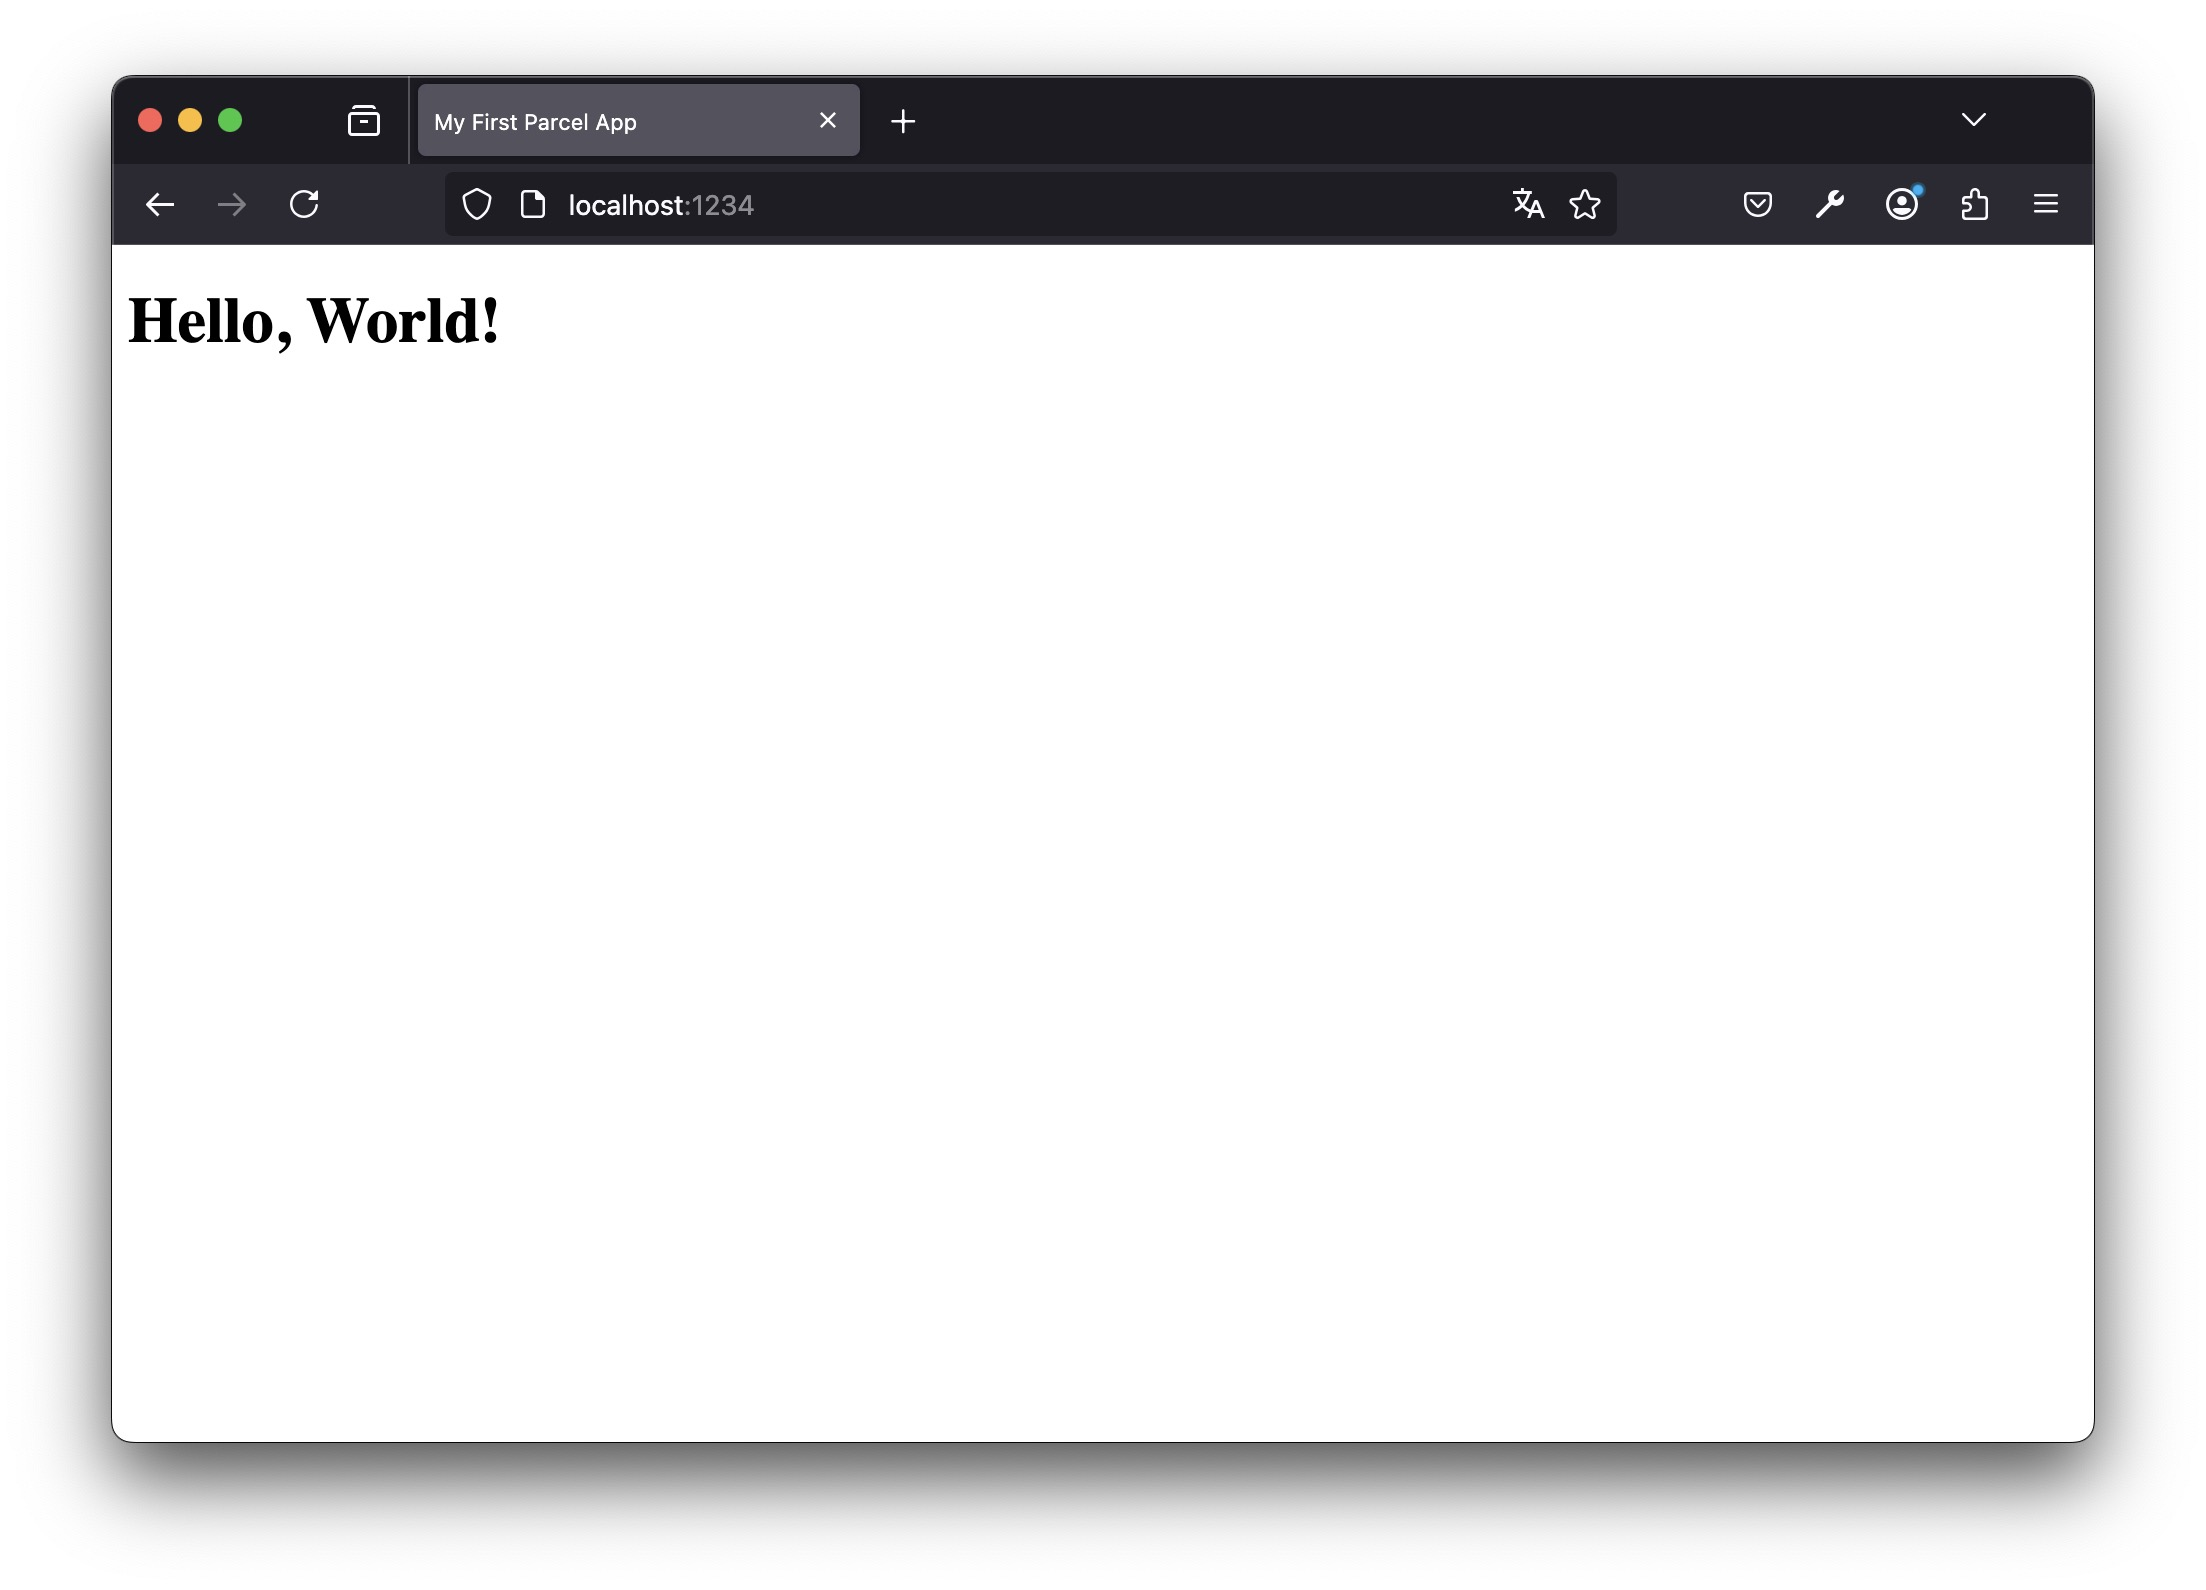
\includegraphics[width=0.8\textwidth]{./img/hello-world}
     \caption{Captura de pantalla de un Hello World básico en HTML}
     \label{fig:hello-world}
 \end{figure}

Se han realizado las modificaciones necesarias para incluir una hoja de estilos y script de ejemplos para comprobar que Parcel las procesa correctamente.
Sin tener que refrescar el navegador, los cambios se han reflejado instantáneamente en la página web (ver Figura~\ref{fig:parcel}).

 \begin{figure}[h!]
     \centering
     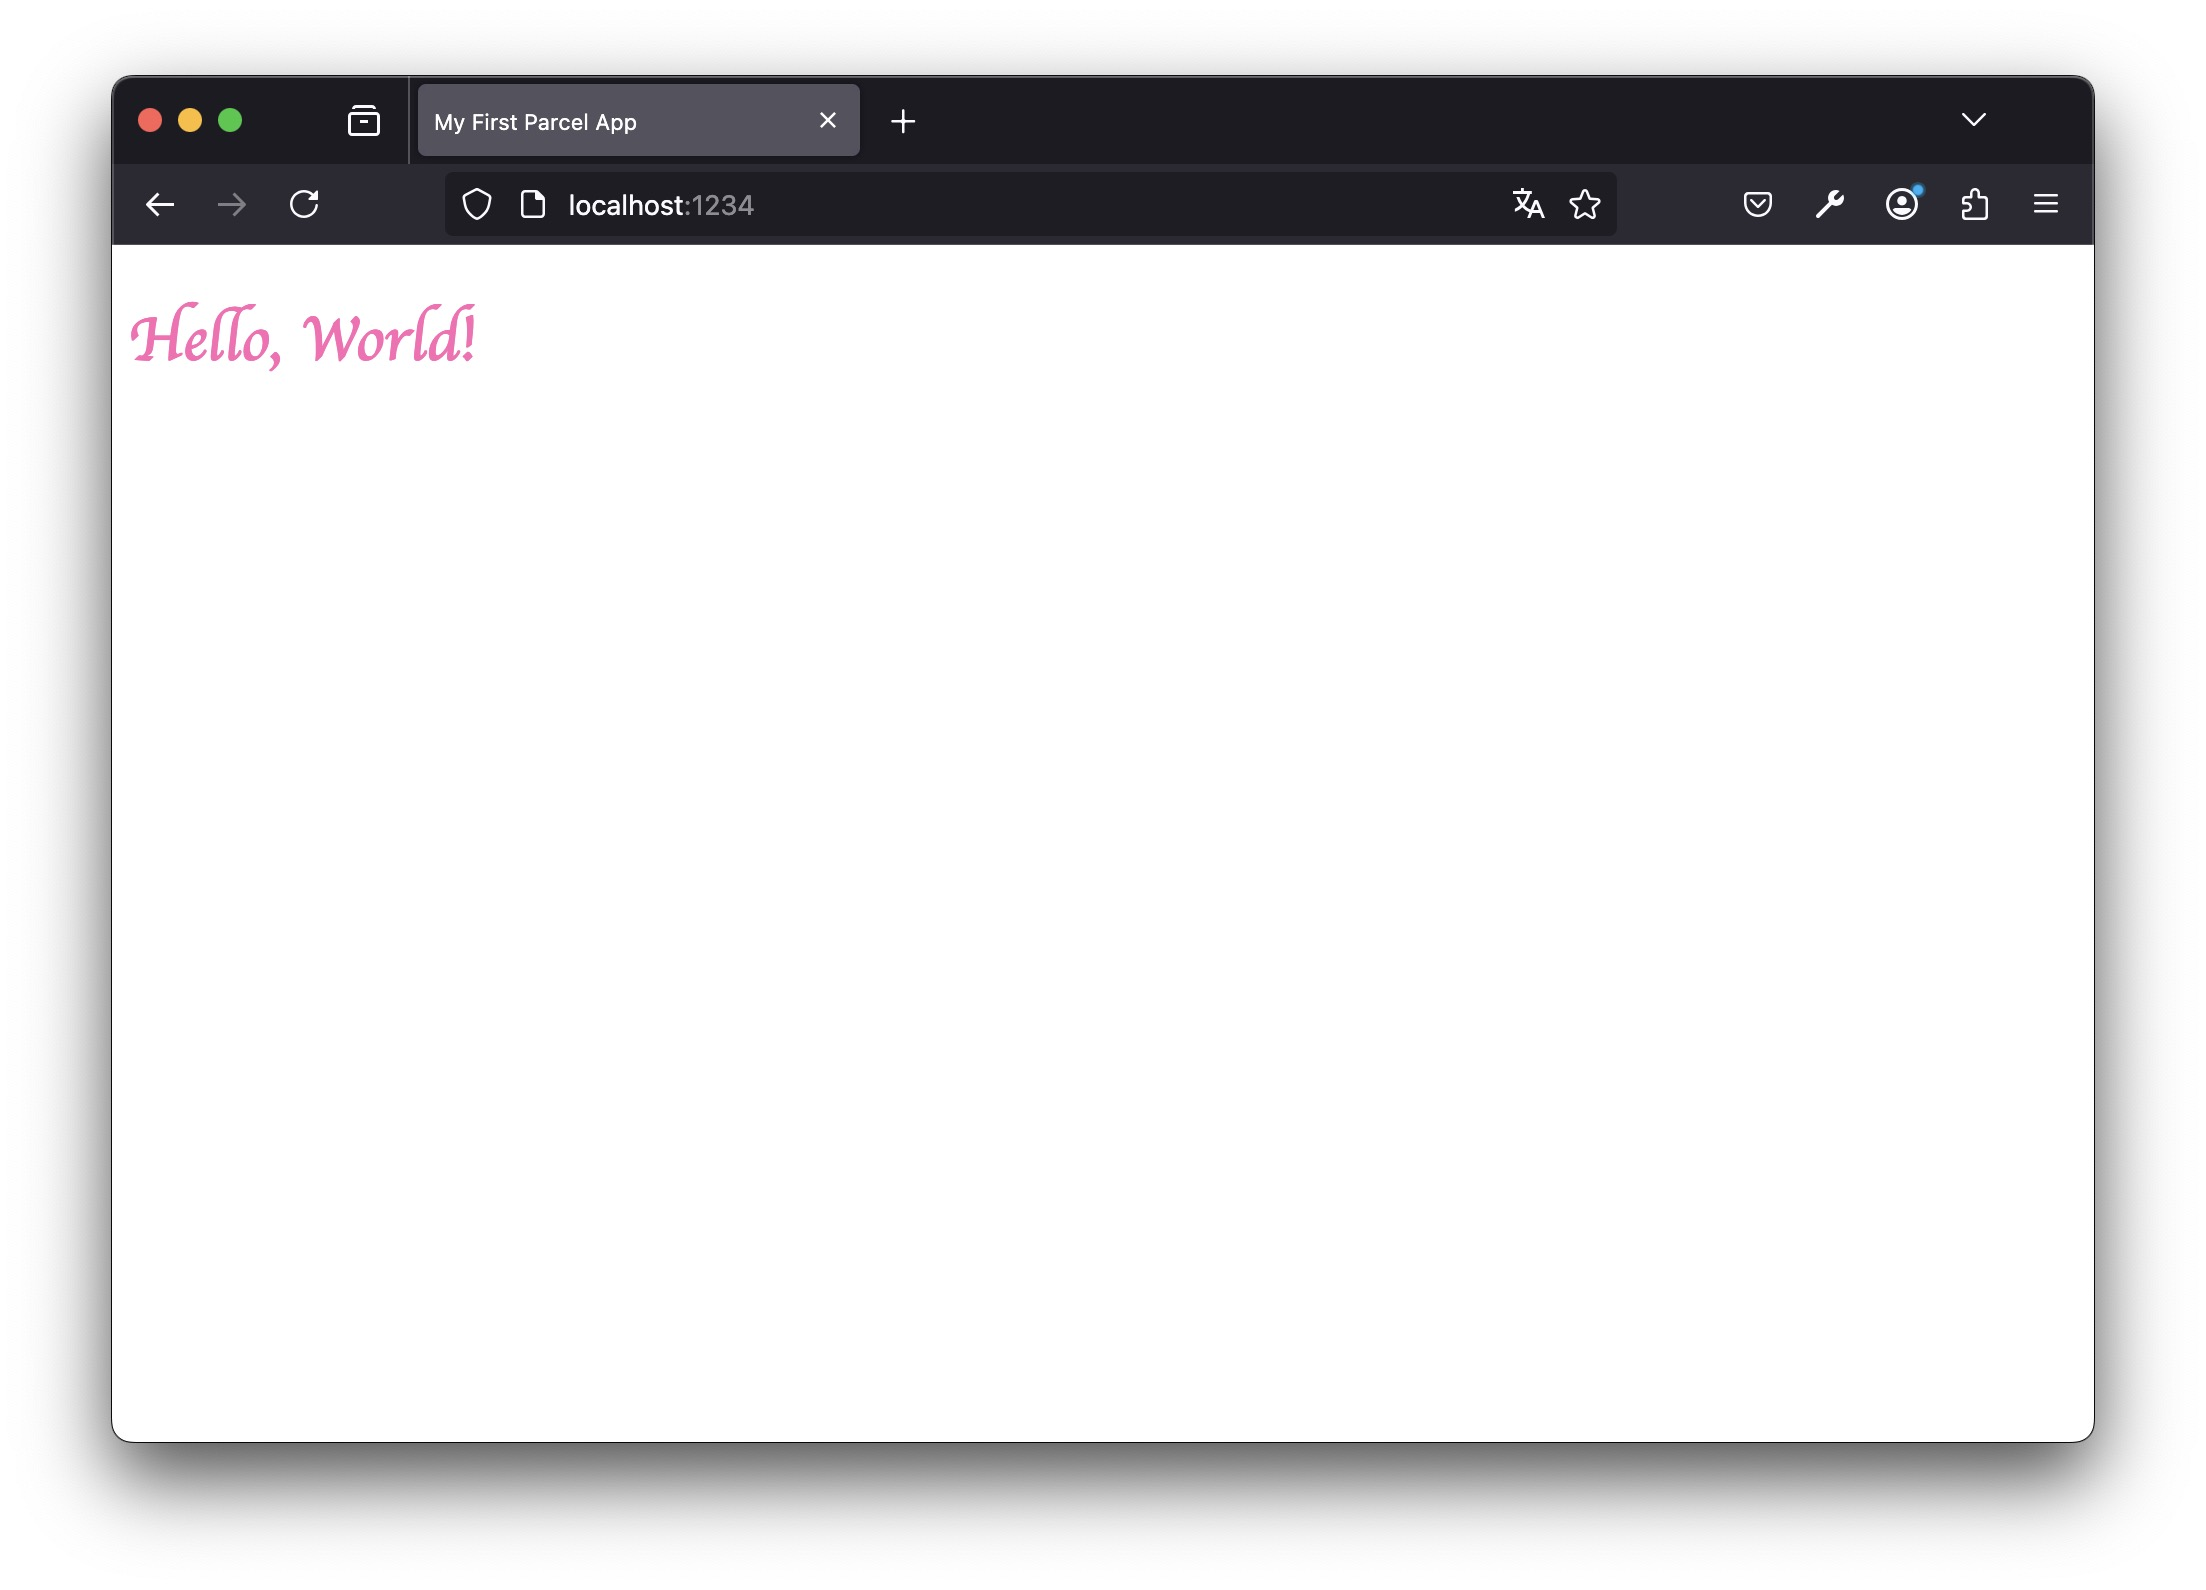
\includegraphics[width=0.8\textwidth]{./img/hello-world-styled}
     \caption{Captura de pantalla de la página web con Parcel}
     \label{fig:parcel}
 \end{figure}

\end{document}
